

\begin{landscape}
\tiny % Utiliza un tamaño de letra más pequeño
\setlength{\tabcolsep}{4pt} % Ajusta el espacio entre columnas
\renewcommand{\arraystretch}{1.5} % Ajusta el espacio vertical dentro de las celdas

\begin{table}[ht]
\centering
\caption{Matriz de Operacionalización: Estimación de parámetros fisicoquímicos para evaluar la calidad del agua en la Laguna de Pacucha mediante geoestadística 2023}
\begin{tabularx}{\linewidth}{|X|X|X|X|X|X|}
\hline
\textbf{Variable} & \textbf{Definición Conceptual} & \textbf{Definición Operacional} & \textbf{Dimensiones} & \textbf{Indicadores} & \textbf{Instrumento} \\
\hline
Calidad del agua & La calidad del agua se refiere a la condición del agua determinada mediante indicadores físicos, químicos y biológicos, evaluados a partir de datos de monitoreo y comparados con estándares específicos \cite{Li2019}. & Medición de parámetros esenciales como temperatura, pH, oxígeno disuelto y conductividad eléctrica en ubicaciones estratégicas de la Laguna de Pacucha, incluyendo áreas próximas a efluentes y afluentes, empleando un equipo multiparamétrico de Hanna Instruments. Estos datos se contrastarán con los Estándares de Calidad Ambiental (ECAs). & Parámetros físicos y químicos. & Temperatura, oxígeno disuelto, pH, conductividad. & Equipo multiparámetro Hanna HI98194 en sitio. \\
\hline
\end{tabularx}
\end{table}
\end{landscape}




\begin{figure}
    \centering
    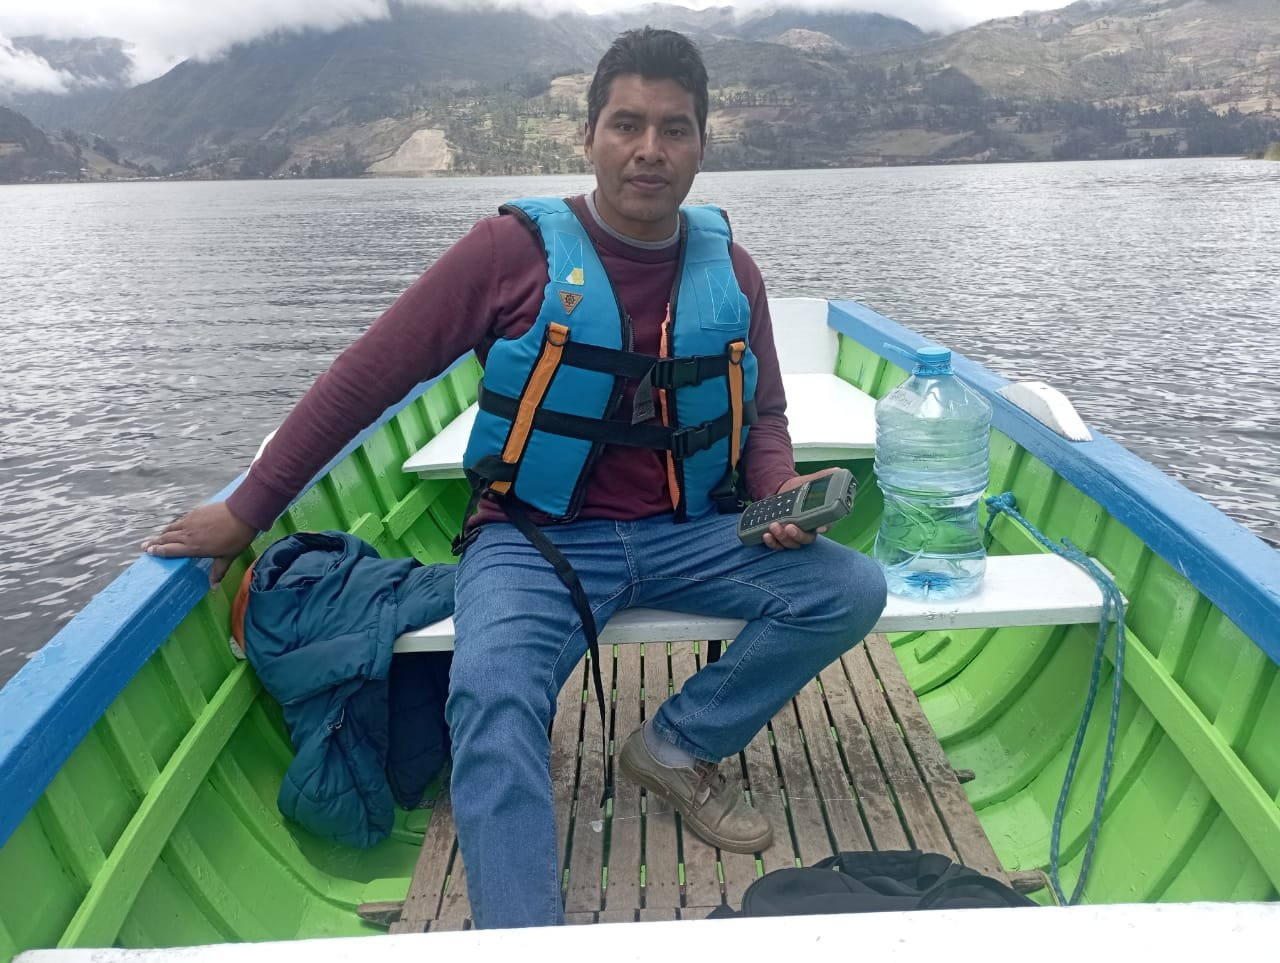
\includegraphics[width=1\linewidth]{Anexos/teybi.jpeg}
    \caption{Recolección de muestras en la Laguna de Pacucha}
    \label{fig:enter-label}
\end{figure}

\begin{figure}
    \centering
    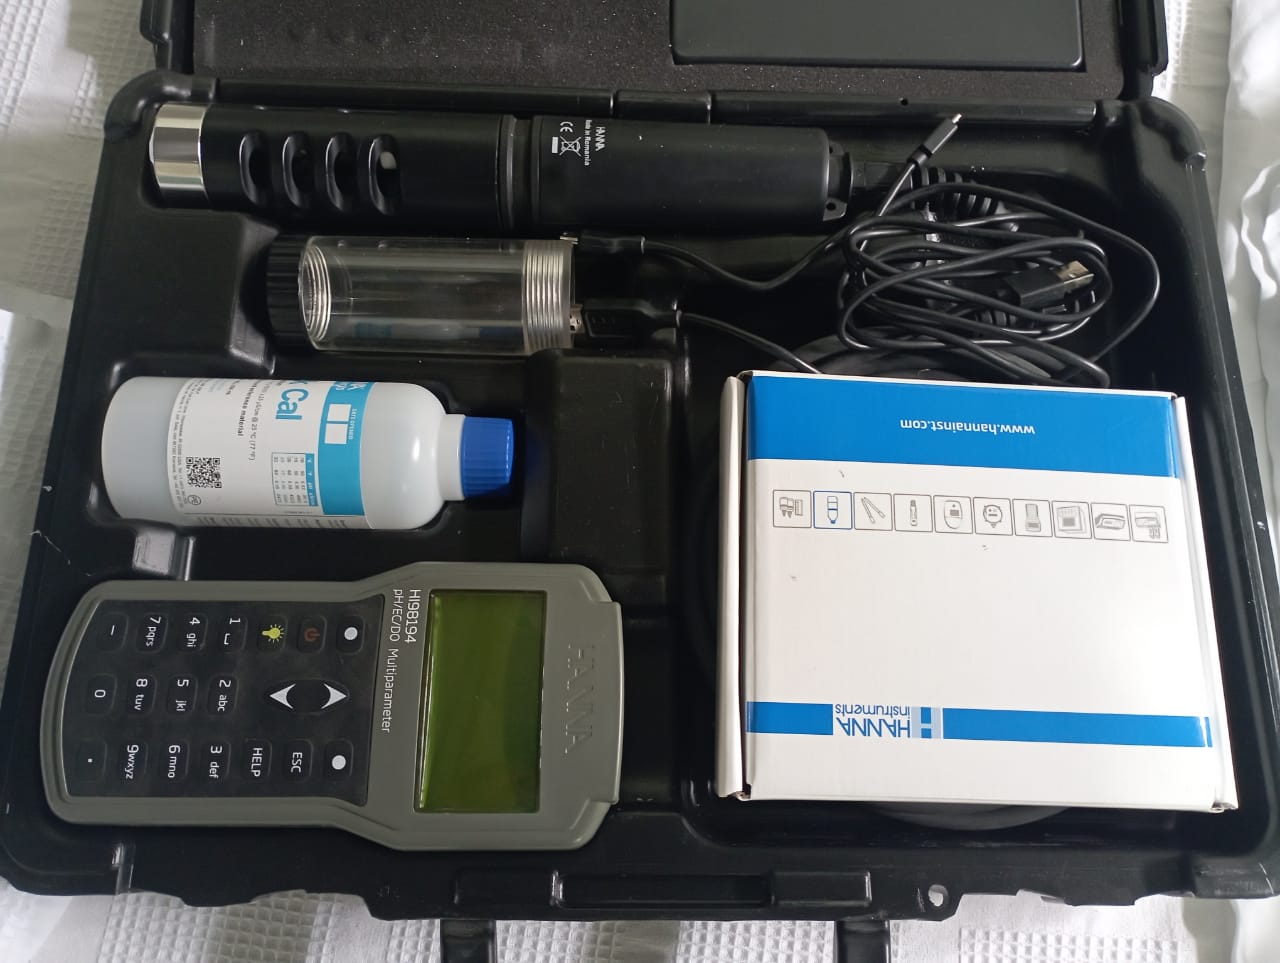
\includegraphics[width=0.7\linewidth]{Anexos/equipos.jpeg}
    \caption{Kit Equipos GPS y Multiparámetro}
    \label{fig:enter-label}
\end{figure}

\begin{figure}
    \centering
    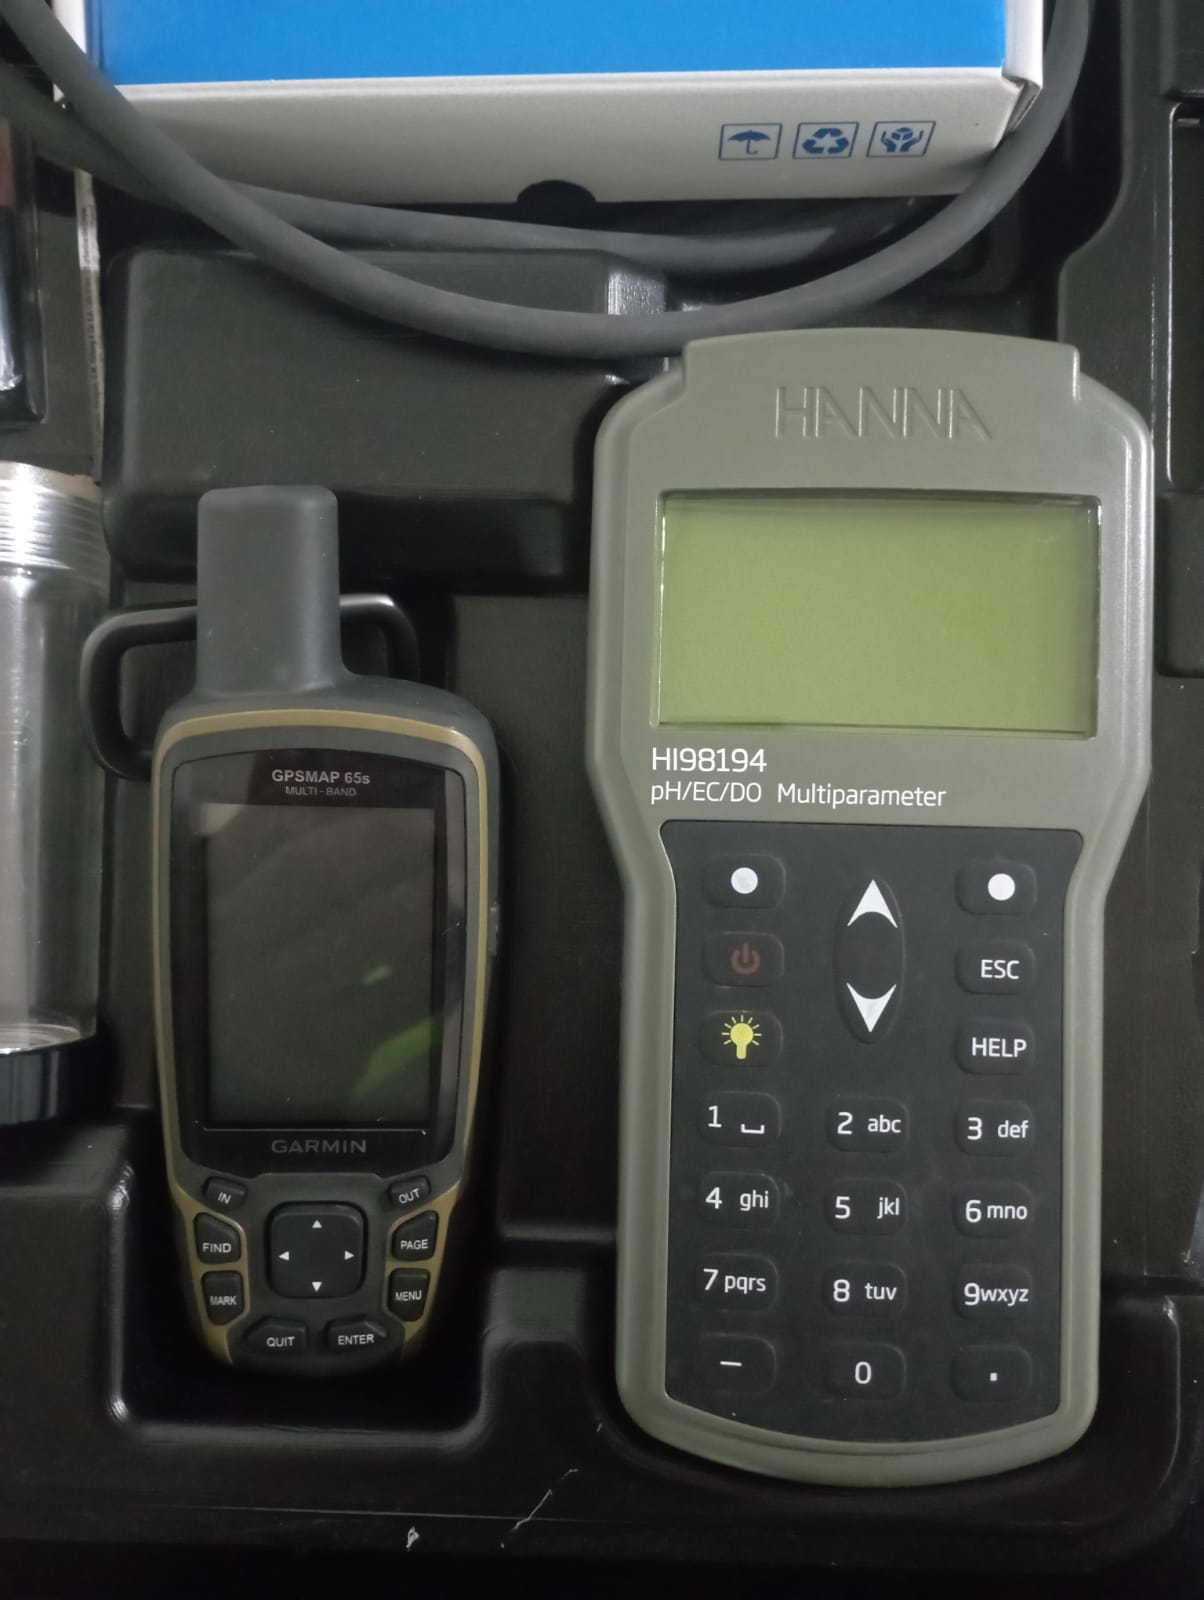
\includegraphics[width=0.8\linewidth]{Anexos/duo.jpeg}
    \caption{Equipos GPS y Multiparámetro}
    \label{fig:enter-label}
\end{figure}

\begin{figure}
    \centering
    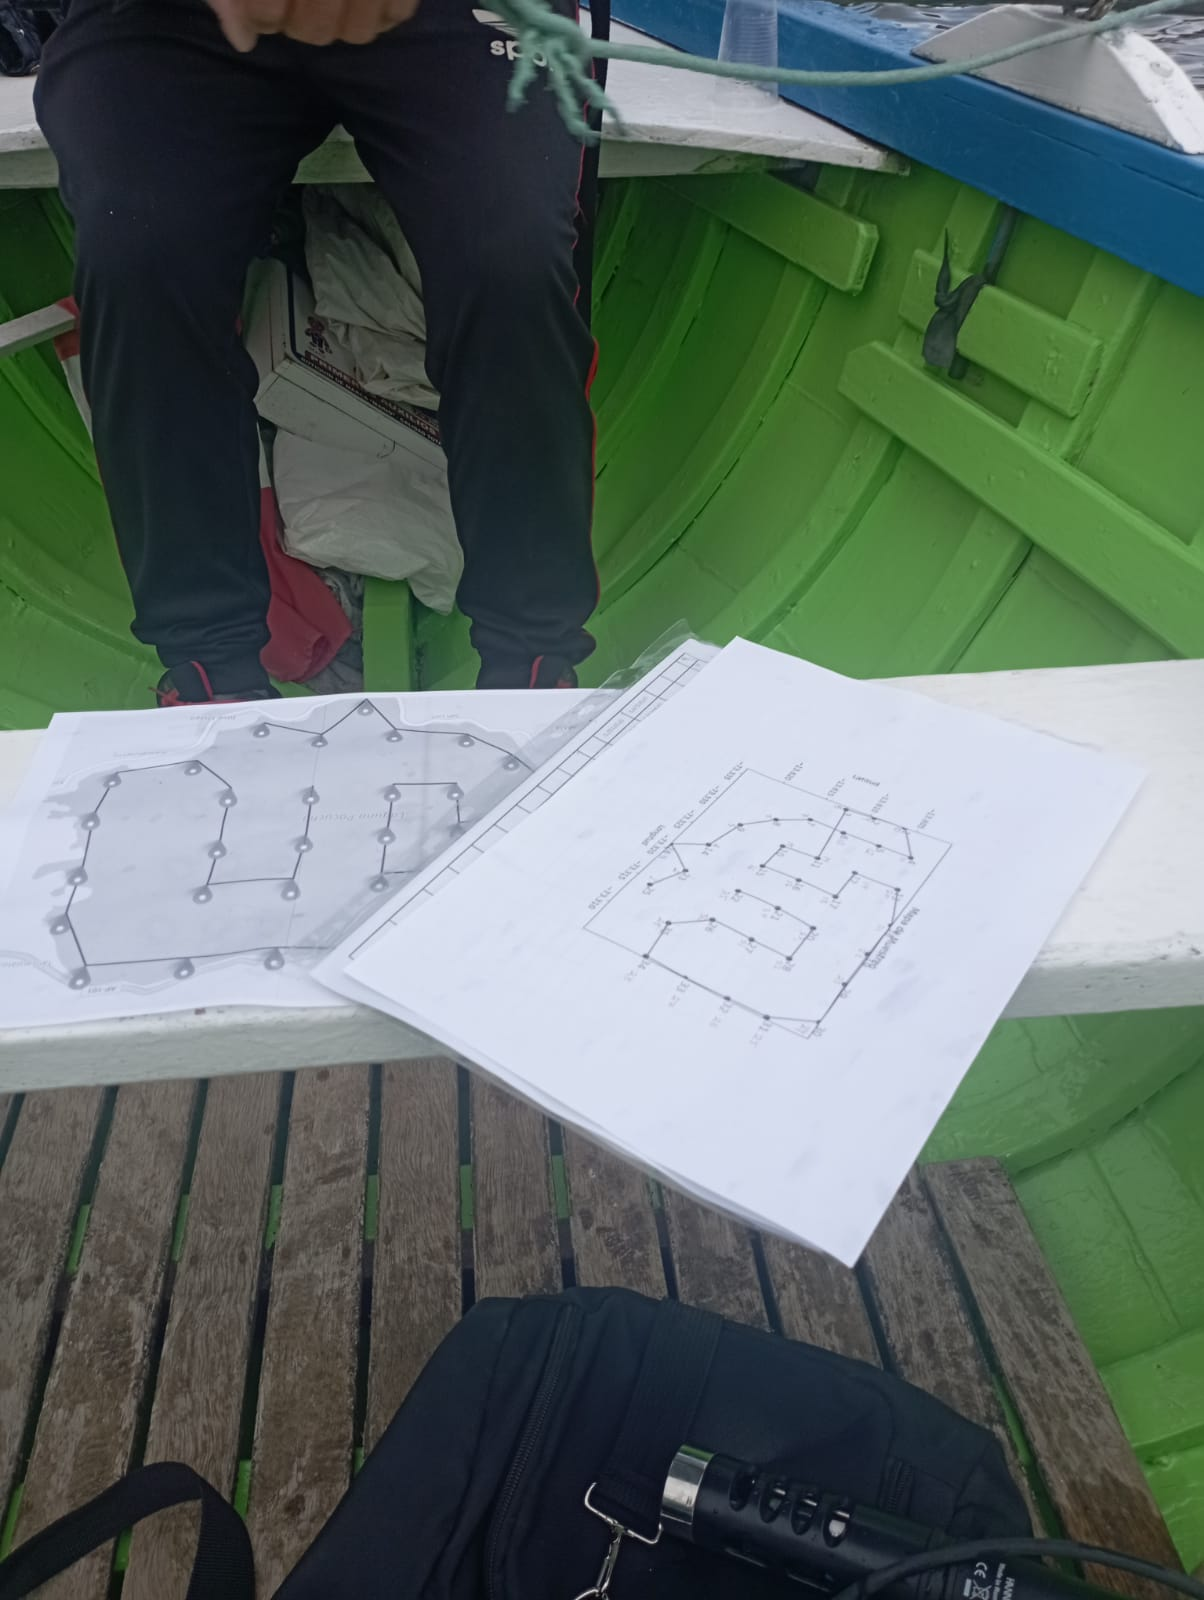
\includegraphics[width=0.7\linewidth]{Anexos/planning.jpeg}
    \caption{Planificación }
    \label{fig:enter-label}
\end{figure}

\begin{figure}
    \centering
    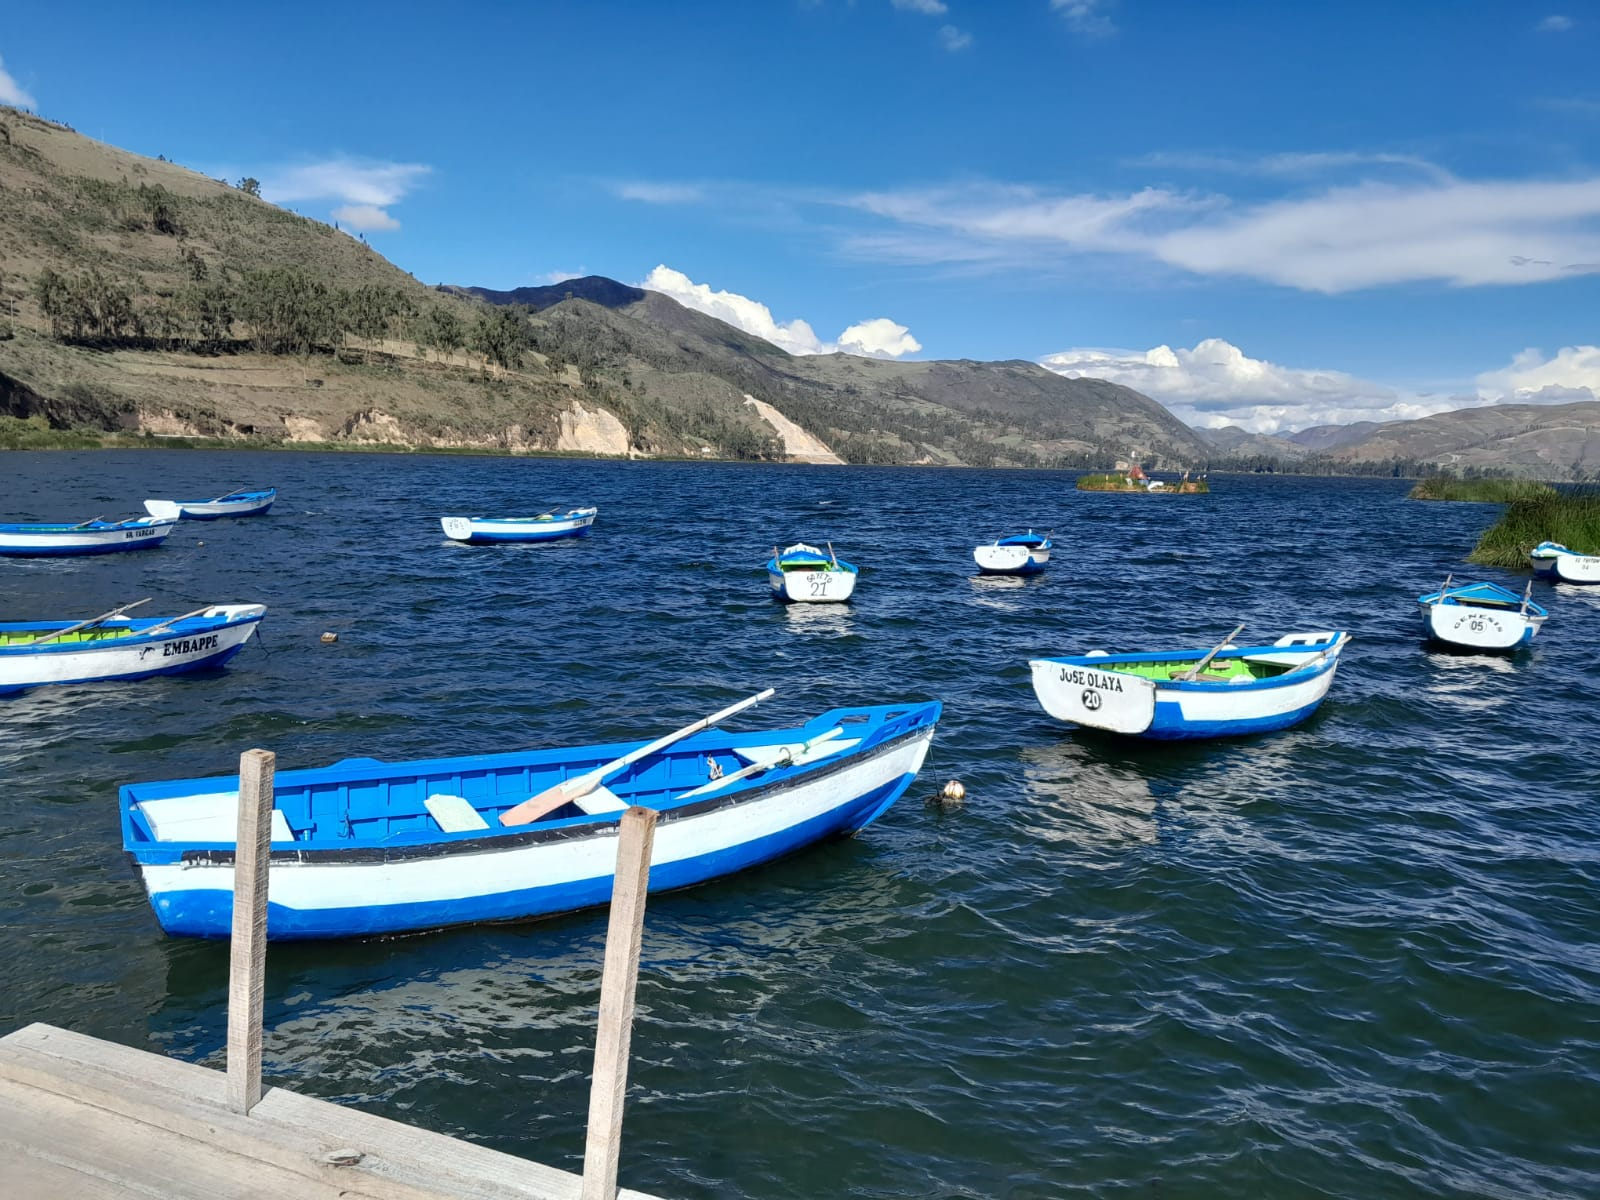
\includegraphics[width=0.9\linewidth]{Anexos/laguna.jpeg}
    \caption{Laguna de Pacucha}
    \label{fig:enter-label}
\end{figure}

\begin{figure}
    \centering
    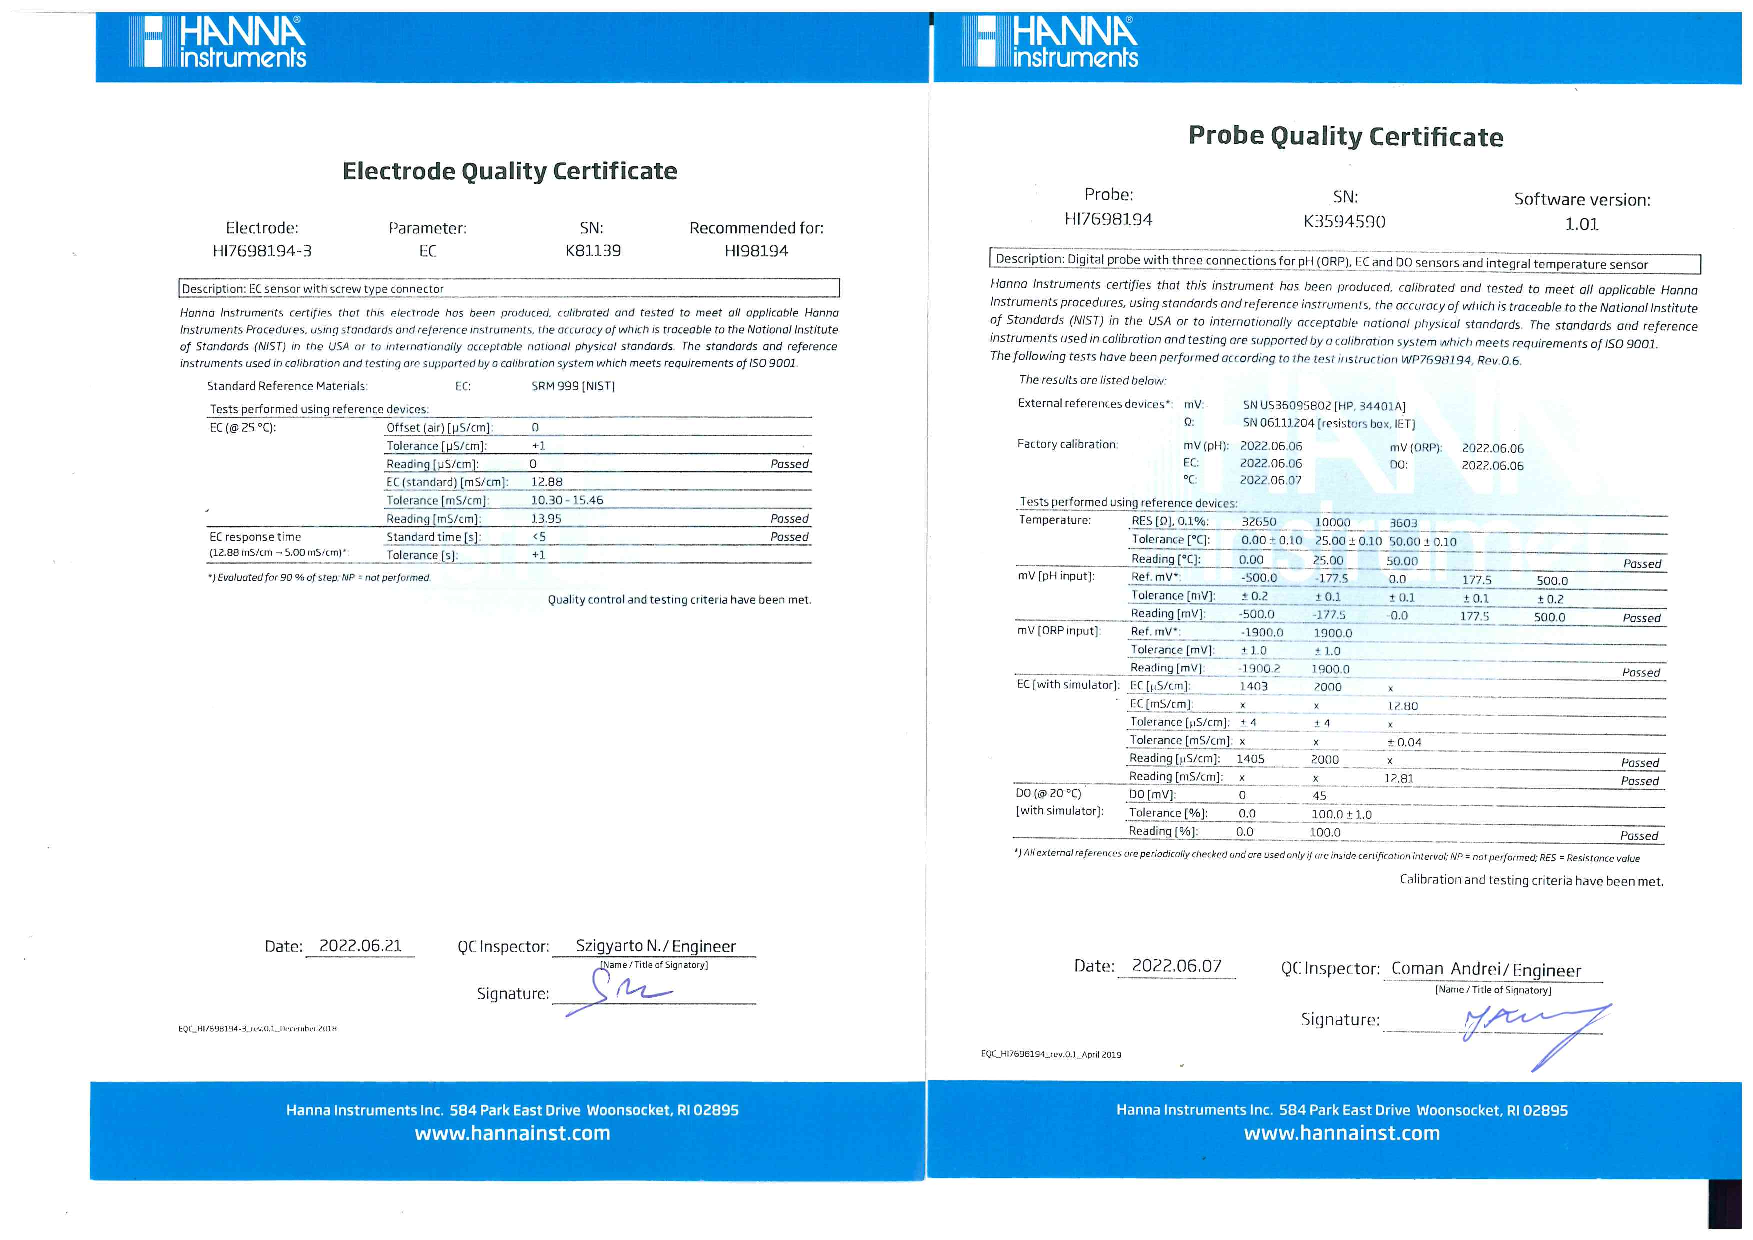
\includegraphics[width=1\linewidth]{Anexos/1.pdf}
    \caption{Certificado Hanna Instrumentos}
    \label{fig:enter-label}
\end{figure}

\begin{figure}
    \centering
    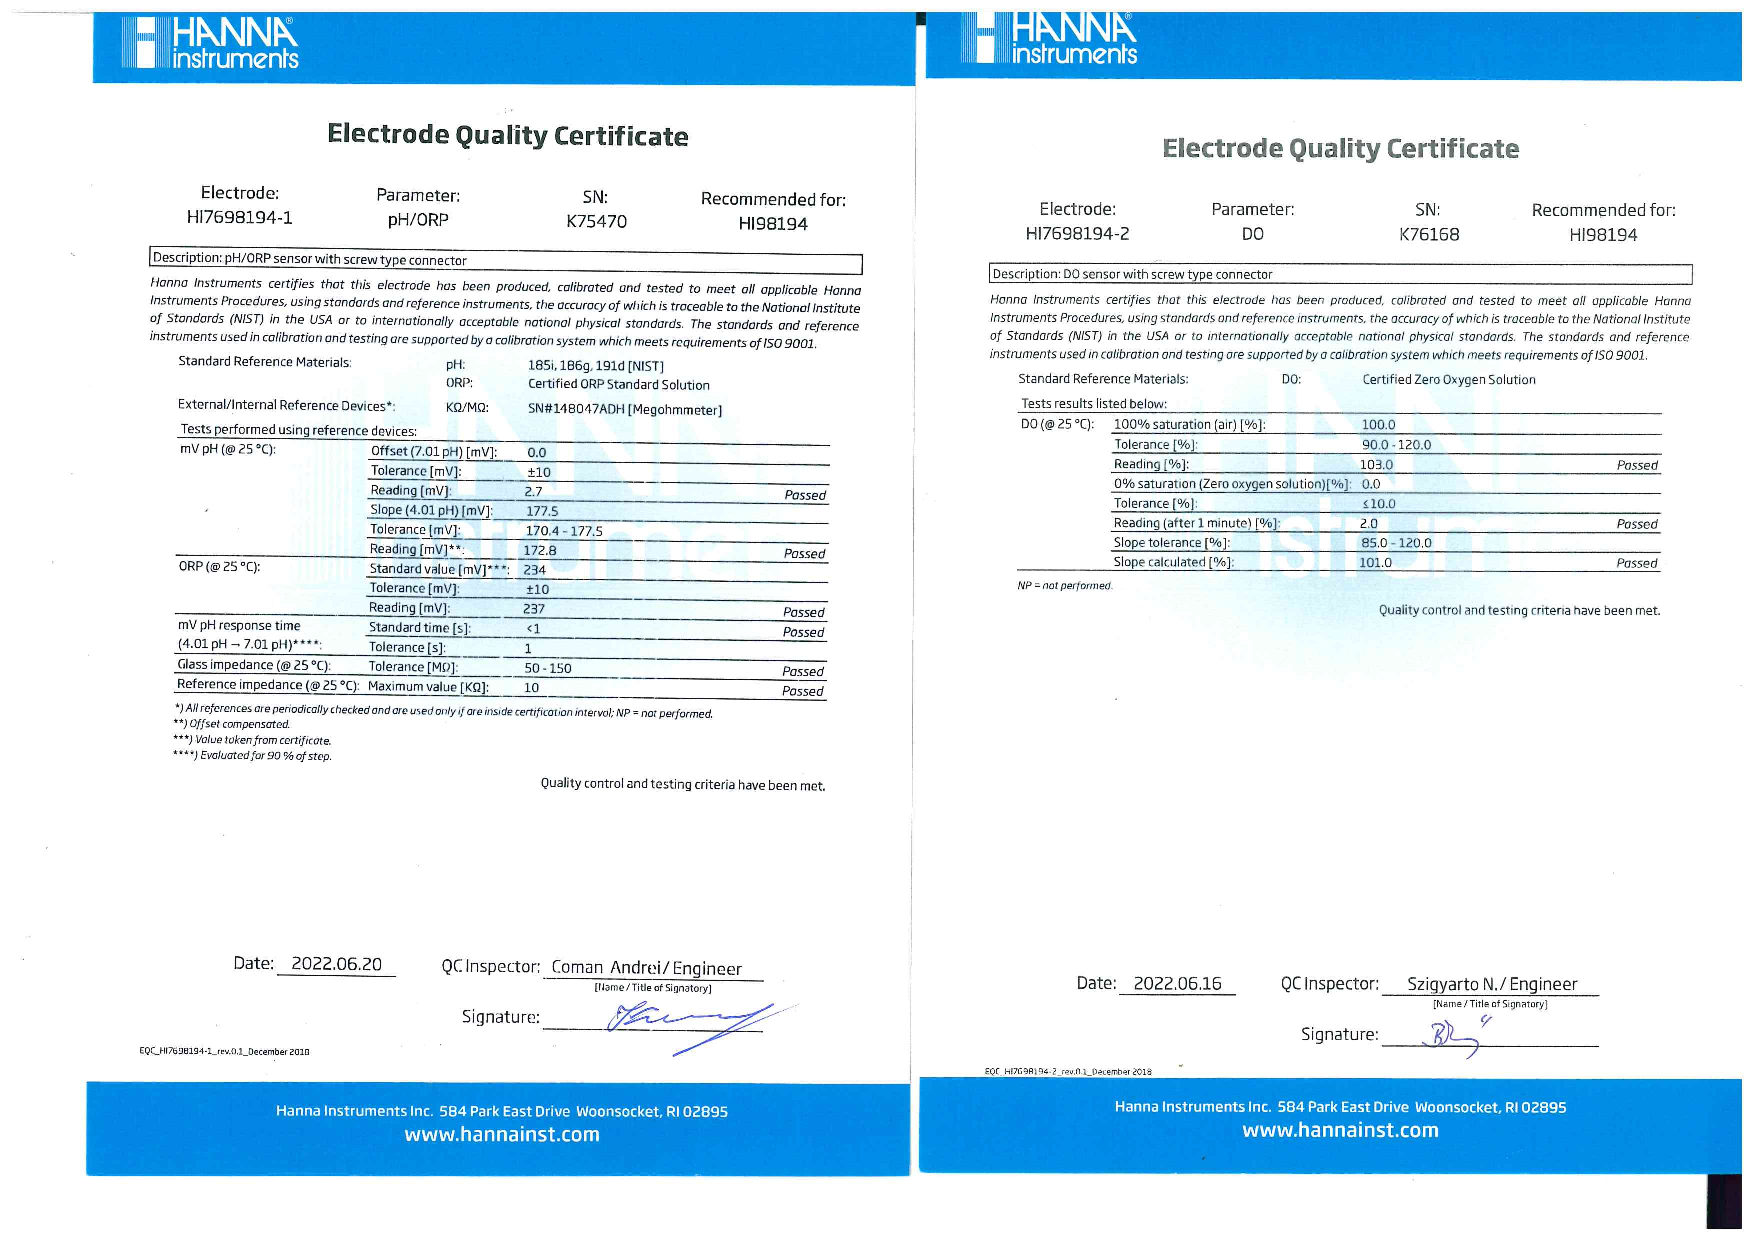
\includegraphics[width=1\linewidth]{Anexos/2.pdf}
    \caption{Certificado Hanna Instrumentos}
    \label{fig:enter-label}
\end{figure}

\begin{figure}
    \centering
    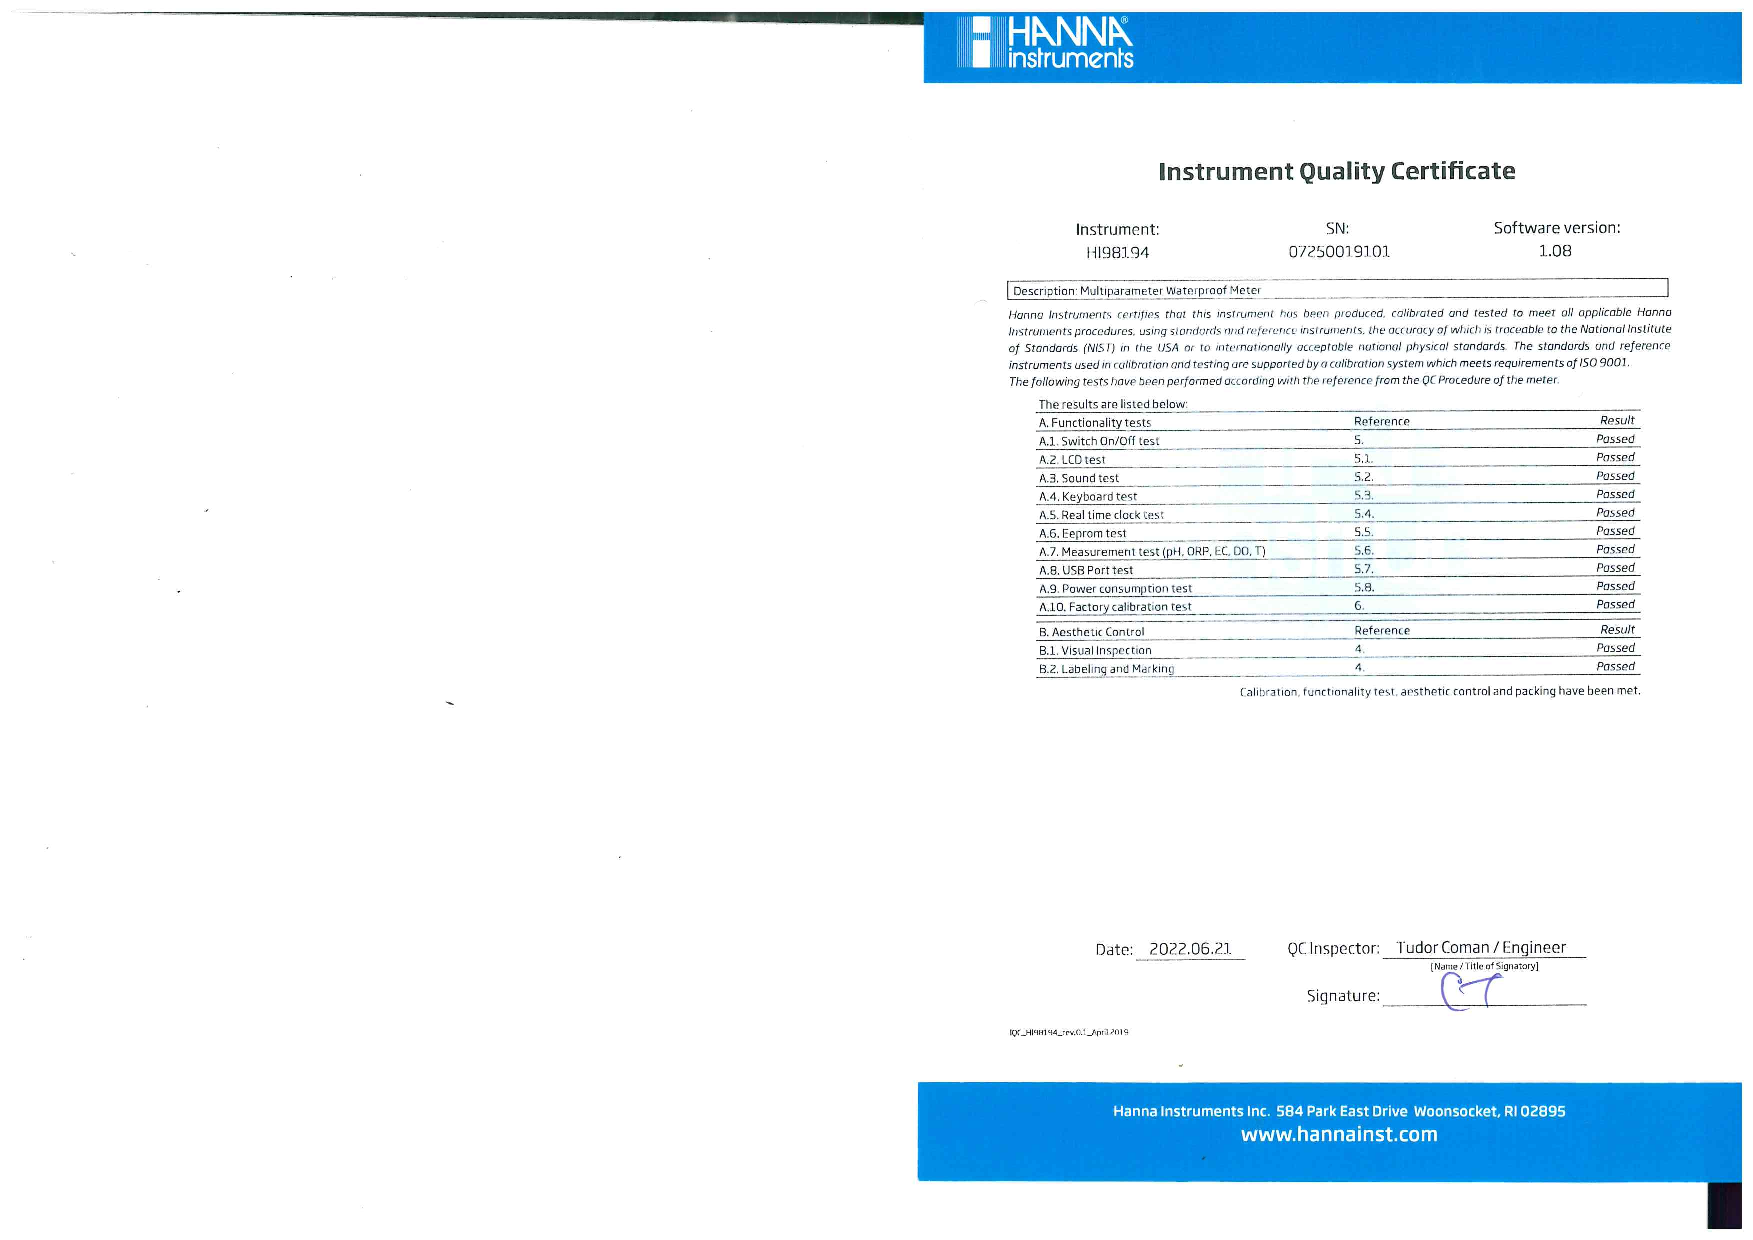
\includegraphics[width=1\linewidth]{Anexos/3.pdf}
    \caption{Certificado Hanna Instrumentos}
    \label{fig:enter-label}
\end{figure}